%% LyX 2.3.5-1 created this file.  For more info, see http://www.lyx.org/.
%% Do not edit unless you really know what you are doing.
\documentclass[onecolumn,english]{article}
\usepackage[T1]{fontenc}
\usepackage[latin9]{inputenc}
\usepackage{float}
\usepackage{graphicx}
\usepackage{todonotes}

\makeatletter

%%%%%%%%%%%%%%%%%%%%%%%%%%%%%% LyX specific LaTeX commands.
%% Because html converters don't know tabularnewline
\providecommand{\tabularnewline}{\\}
%% A simple dot to overcome graphicx limitations
\newcommand{\lyxdot}{.}


\makeatother

\usepackage{babel}
\begin{document}
\title{Prediction of Protein-Protein Interactions on the Human and
Rice Interactome}
\author{Nicol\'as Antonio L\'opez Rozo}
\maketitle
\begin{abstract}
Previous Network-based efforts to predict unmapped protein-protein interactions (PPI's) suggest that proteins with multiple paths of length~3 (L3) are more likely to be connected. This paper extends this so-called L3 principle by taking into account feature extraction and using \texttt{XGBoost} techniques for prediction. In particular, we train the model using handcrafted features as well as features learned from embeddings using \texttt{Node2Vec}. Our main result shows that while L3 remains an important principle for predicting links, the approach is outperform by using embedded features. The mentioned approaches are compared using the human and the rice interactomes.

% need include a feature that compares the dimension of the embedding is useful for prediction with L3 to show that they independent measures - we do not want to be learning L3 through node2vec
\end{abstract}


\section{Introduction}
% need to add other relevant references 
Proteins, as a fundamental constituents of any living being and their
``building blocks'' in terms of biological functionality, interact
among themselves and with other molecules according to their amino
acid sequences and specific three-dimensional structure and folding.
These interactions also depend on many physical and chemical properties
of each macro-molecule and on the cellular organelle where they operate,
such as pH and temperature. For this reason, experimental ways to
reproduce all of the necessary conditions to validate if an interaction
actually occurs within the cell are generally expensive.

The most common way to validate PPI's is the \emph{Yeast-Two-Hybrid}
technique (also known as \emph{two-hybrid screening} or \emph{Y2H}),
which is based on the expression of a specific reporter gene that
activates by the binding of a DNA-binding Domain (DB) and an Activation
Domain (AD) of a Transcription Factor. For the Y2H technique, a protein
is fused to the DB domain (known as \emph{bait}) and another one to
the AD (known as \emph{prey}). If the proteins do not interact, then
the reporter gene is not expressed. Otherwise, the reporter gene expression
is activated by the activation domain.

\begin{figure}[h]
\caption{Yeast-2-Hybrid Technique}

\noindent \centering{}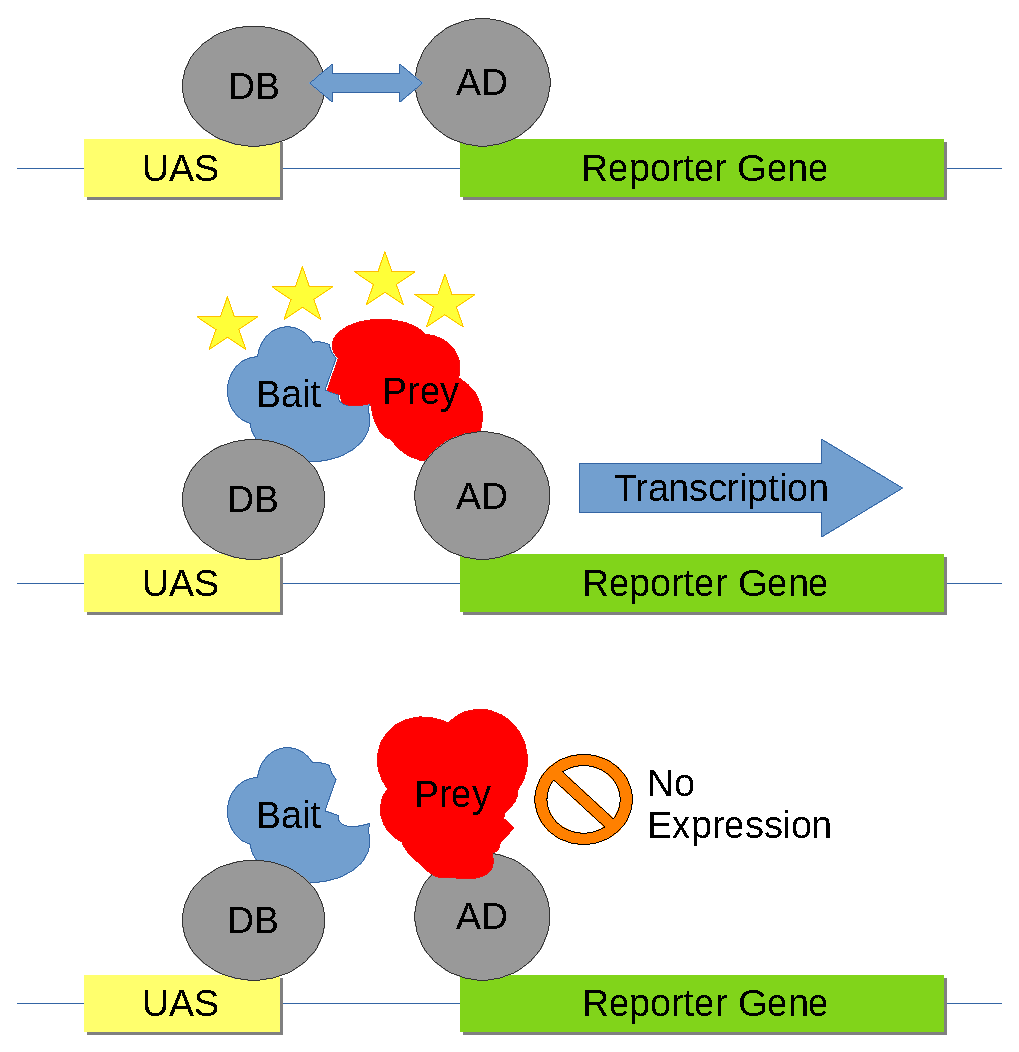
\includegraphics[width=1\columnwidth]{Y2H}
\end{figure}

Having several of these Y2H results allows scientists to establish
a PPI network, where all known interactions for each protein are represented.
Several algorithms are proposed over these networks in order to predict
unknown interactions. In this report, three prediction methods are
presented and their results are shown: Common Neighbors (\textbf{CN}),
which uses the length-2 path count; length-3 path count (\textbf{A3});
and degree-normalized length-3 paths score (\textbf{L3}).

\begin{figure}[h]
\caption{Protein-Protein Interaction Prediction Scheme}

\noindent \centering{}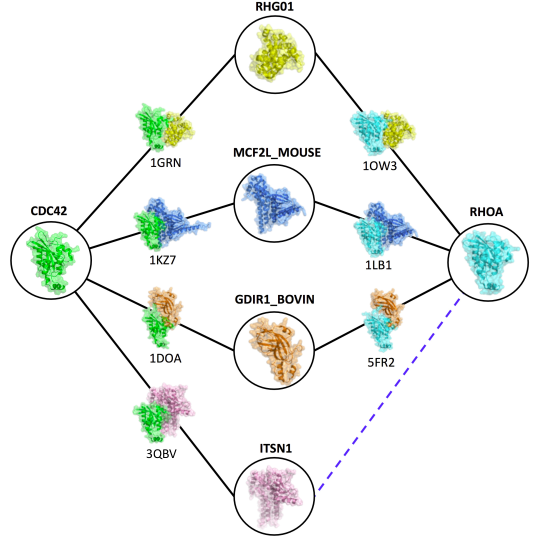
\includegraphics[width=0.9\columnwidth]{PPI_prediction}
\end{figure}

Focus of the present study is to evaluate different methods for predicting
protein-protein interactions (PPIs) using the existing knowledge of
the network, which is an undirected graph. The traditional way is
usually based on social networks analysis, more specifically on the
Triadic Closure Principle (TCP), that states that the more common
shared friends that two people have, the more likely that they know
each other. As shown in the next sections, the mentioned approach
fails because it does not consider the structural and chemical properties
of the proteins.

For achieving the described results, several networks are used and
compared using state-of-the-art methods, as well as the proposed ones
(CN, A3, L3). For this report, the human interactome was used (\emph{HI-II-14}).
A curated version of the mentioned network (\emph{HI-TESTED})
was also used in order to compare the influence of research bias on
the network predictions. A massive experimental assay was carried
on and its results are consolidated and used to build a validation
network (\emph{HI-III}).

\section{Materials and Methods}

\subsection{Data Availability}

Human interactome data and base source code were downloaded from the
repository of the length-3 degree normalized paths methodology~\cite{Kovacs2019}:
the dataset \emph{HI-II-14} and \emph{HI-TESTED} are used
for prediction and the dataset \emph{HI-III} is used for validation.
Rice interactome information was downloaded from the STRING database~\cite{Szklarczyk2019}, corresponding to the \emph{Oryza sativa} subspecies.
The downloaded file was \emph{4530.protein.links.detailed.v11.0.txt}.
and contains more than 8 million PPIs from several resources. For
the purpose of this study and based on the previous work, only PPIs
with evidence from curated databases were used (rows where \emph{databases}
column has a value greater than zero), resulting in a network with
NNNN nodes and MMMM edges.

\subsection{Code Implementation}

Previous code implementation was adapted from \texttt{C++} to \texttt{Python}
(3.6), in order to unify the algorithms into one single script. For
the purpose of algorithmic validation, the three methods were implemented
from scratch with basic functionalities and data structures of the
\emph{Python} (V3.6) language.

\subsection{Data Preprocessing}

Information for the human interactome was used as-is, which corresponds
to networks of $4298$, $3727$ and $5604$ proteins and $13868$,
$9433$ and $23322$ interactions. For the rice interactome, an additional
preprocessing was performed. The filtered network for rice consists
of $5025$ proteins (nodes) and $164420$ interactions (edges) distributed
among $178$ connected components. The connected component with the
greatest number of edges was selected in this case. 

The extracted connected component consists of $n=4390$ nodes and
$m=163319$ edges, which corresponds to $99.33%\%
$ of filtered edges. Further investigation is applied to this network,
which is very similar in number of nodes to the curated information
on the human interactome, although rice network is much more connected.

\subsection{Edge Prediction}

For the interaction prediction for each network, the algorithms described
below were used. It is important to keep in mind how the protein-protein
interaction (PPI) network $G=(V,E)$ is conceptualized: each node
($v_{i}\in V$) represents a protein and each undirected edge ($e_{b}=\{v_{i},v_{j}\},\,e_{b}\in E$)
represents and interaction among proteins $v_{i}$ and $v_{j}$.

\begin{figure}[h]
\caption{Edge Prediction Paradigms}

\noindent \centering{}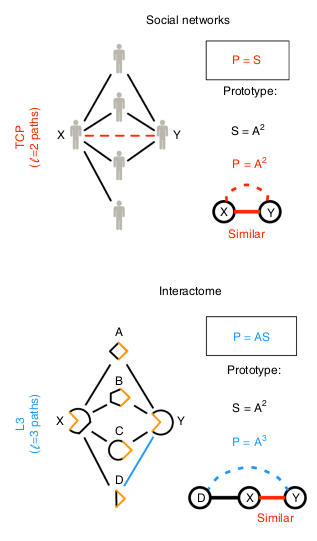
\includegraphics[width=0.8\columnwidth]{TCP_extract.png}
\end{figure}

\begin{description}
\item [{Common~Neighbors~(CN)}] This method is based on the Triadic Closure
Principle: ``the more common friends two individuals have, the more
likely that they know each other''. For the implementation of this
method, $A{{}^2}$ matrix is calculated, being $A$ the adjacency
matrix of the network.
\item [{Length-3~Paths~(A3)}] This is the simplest implementation of
the proposed insight of ``if my friends and your friends interact,
then we might interact too''. The calculating is carried on with
$A{{}^3}$, i.e, the third power of the adjacency matrix.
\item [{Degree-normalized~L-3~Score~(L3)}] The previous approach might
overestimate the importance of some edges due to intermediate hubs
which add many shortcuts in the graph. To address that issue, a degree
normalization for the path $X\rightarrow U\rightarrow V\rightarrow Y$
is applied by considering the degree $k$ of the intermediate nodes
$U$ and $V$, as follows.
\[
p_{XY}=\sum_{U,V}\frac{A_{XU}\cdot A_{UV}\cdot A_{VY}}{\sqrt{k_{U}\cdot k_{V}}}
\]
\\
where $A_{ij}$ represents the value of the adjacency matrix for nodes
$i$ and $j$: 1 if the edge $\{i,j\}$ exists, 0 otherwise.
\end{description}

\subsection{Sampling and Precision Counting}

Sampling proceeds as follows: first, a fraction (10\%) of the edges
is removed at random from the network. Then, for each method (\textbf{CN},
\textbf{A3}, \textbf{L3}) the prediction of the removed fraction is
performed. The new edges are then compared against the original (removed)
edges according to the ranking that each method yields. Edges belonging
to the original connected component are considered positive in the
sense that they are experimentally validated interactions. For each
of the tested networks and a rank $r$, the precision was calculated
as 
\[
P_{r}=\frac{L_{r}}{r}
\]
\\
where $L_{r}$ is the total number of positive edges in the range
$[1,r]$.

The previous procedure was applied for a fraction of 0.90 remaining
edges, and a mean of 10 simulations was obtained.

\subsection{Feature Extraction with \texttt{Node2Vec}}

The \texttt{Node2Vec} module was used for extracting features of the
rice interactome graph. The parameters and considerations for the
model were:
\begin{itemize}
\item All paths in the random walks are equally likely (\texttt{p=1, q=1})
\item Use a modest number of dimensions and threads for calculation (\texttt{dimensions=16,
workers=4})
\item Since length-3 paths are the defining property in this study, there
is no necessity for longer walks. However, it is important to try
out many possible redundant routes and to consider a window of at
least 4 (\texttt{walk\_length=5, num\_walks=300, window=5})
\item Other standard parameters were left with default values (\texttt{min\_count=1,
batch\_words=4})
\item Edge embeddings were calculated using a geometric ratio of the node
embeddings (\texttt{HadamardEmbedder})
\end{itemize}

\subsection{Handcrafted Feature}

Due to the poor results of the \emph{raw} Length-3 counting (\textbf{A3}),
a different approach for this information was carried out in the present
study: As it still gives a lot of information that might be useful
for a predictive routine, this counting was normalized (dividing by
the greatest counting in the \textbf{A3} top predictions) and then
used as a feature for the Machine Learning algorithm. For completeness,
also \textbf{CN} and \textbf{L3} information was used as a possible
feature. Finally, the case were no handcrafted feature was also considered,
that is, only the features extracted from the structure of the network.

\subsection{Feature to Predict: Existence}

The feature to predict corresponds to the possible existence (\emph{True/False})
of a link based on the existing information of the network, using
the network itself in a random sub\_exploration (\texttt{Node2Vec})
as well as in a structured search (A3). This property is evaluated
by taking out a fraction of the edges and then trying to predict for
a given set of possible edges if they have a high probability to belong
to the original network.

\subsection{Machine Learning Algorithm}

The Extreme Gradient Boosting implementation of gradient boosted trees
is applied in this study to evaluate the existence of an edge. Gradient
boosted trees are usually used for supervised learning problems, where
the training data $X_{i}$ has multiple features and pretends to explain
(or predict) a target variable $Y_{i}$. The corresponding implementation
applied for this study is \texttt{XGBoost}, available publicly.

The selected parameters for the model were \texttt{max\_depth=3}, \texttt{colsample\_bytree=0.6}
and \texttt{eval\_metric=`auc'}.
\subsection{Result Validation}

For applying the test results, a partition of the whole dataset was
made: 80\% of the data was randomly selected and used for training,
while the remaining 20\% was used for validation. The whole training-validation
procedure was applied 5 times.

The chosen metric for validation was the Area under the Curve (\textbf{AUC})
of the Receiver Operating Characteristic (\textbf{ROC}). This curve
corresponds to plot the sensitivity (probability of predicting a real
positive as positive) against 1-specificity (probability of predicting
a real negative as positive). It is worth to remind that AUC values
move in the range $[0,1]$, where 1 is a perfect prediction and 0.5
corresponds to a random guess. Normally, values over 0.8 of AUC are
considered good.

\section{Results}

As explained above, the precision trend for each of the networks are
presented for the predicted top 2000 interactions.

\begin{figure}[h]
\caption{Methods Comparison for \emph{HI-II-14}}

\noindent \centering{}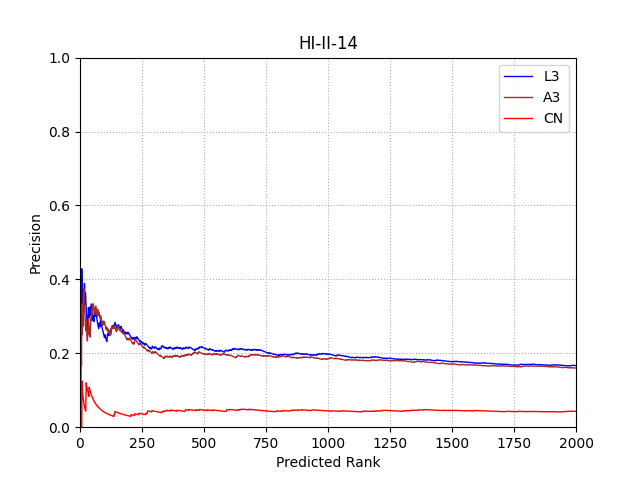
\includegraphics[width=1\columnwidth]{hi-ii-14.png}
\end{figure}

\begin{figure}[h]
\caption{Methods Comparison for \emph{HI-TESTED}}

\noindent \centering{}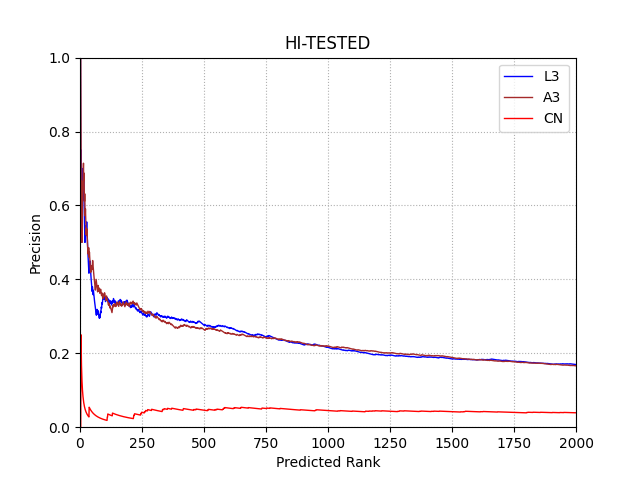
\includegraphics[width=1\columnwidth]{hi-tested.png}
\end{figure}

As it can be inferred from the plots, L3-based predictions outperform
their $A{{}^2}$ counterparts. Results also show that L3-score and
$A^{3}$predictions follow a very similar trend. 

When analyzing the robustness of each of the networks, the following
values for the Weighted Spectral Distribution were found. For a robustness
reference, the Erdos-Renyi model was used to generate a random network
with the same number of nodes and edges and on those random networks,
the WSD was measured.
\begin{center}
\begin{table}[H]
\caption{Validation of Weighted Spectral Distribution}

\centering{}%
\begin{tabular}{|c|c|c|}
\hline 
Network & Network WSD & Erdos-Renyi WSD\tabularnewline
\hline 
\hline 
HI-II-14 & 393.4939 & 198.7706\tabularnewline
\hline 
HI-TESTED & 423.3902 & 276.1065\tabularnewline
\hline 
HI-III (VALID.) & 373.9369 & 153.5329\tabularnewline
\hline 
\end{tabular}
\end{table}
\par\end{center}

The table shows that the three networks used in this report are robust,
because the are significantly more robust than a network with the
same density generated randomly.

\section{Conclusions}

Taking into account the different results validated in this report,
one can conclude that length-3 path methodologies might work better
on protein-protein interactions than its traditional length-2 (TCP
based) counterparts. On the other hand, it can be seen that degree-normalization
has little effect on the predictions, i.e., non-normalized $A{{}^3}$
matrix predictions are still a good methodology for edge prediction
on PPI networks.

Previous result comes as no surprise when the biological basis of
protein interactions is considered: It is necessary that protein A
and protein B have complementary structures in order to interact,
and when classical paths of length~2 are used, the predicted protein
interactions usually have the same structures, and not complementary
ones.

% please update the conclusions - WSD does not seem relevant 
For the analyzed networks, it is also important to highlight their
robustness when compared to a random network with the same density:
if weighted spectral distribution (WSD) is used, then the used networks
are on average twice as robust as their random network versions.

\bibliographystyle{plain}
\bibliography{refs.bib}

\end{document}
